\chapter{Wielowymiarowy regulator PID}
\label{pro_pid}

W ramach kolejnego zadania zaimplementowaliśmy wielowymiarowy regulator 
PID o 4 wejściach i 3 wyjściach. 

\section{Implementacja wielowymiarowego regulatora PID}
\label{pro_pid_implementacja}

Implementacja regulatora wielowymiarowego
jest podobna do zwykłego regulatora jednowymiarowego, z tą różnicą
że każdy parametr skalarny $K_{\mathrm{p}}$, $T_{\mathrm{i}}$ i $T_{\mathrm{d}}$
jest teraz wektorem o takiej ilości elementów jaka jest liczba wejść. \\

\begin{lstlisting}[style=custommatlab,frame=single,label={pro_pid_parametry},caption={Przykładowa definicja parametrów regulatora},captionpos=b]
%% Parametry regulatorow ciaglych
K = [1 0 1 1];
Ti = [3 99999 99999 100];
Td = [0.05 0 0 0];

%% Parametry regulatorow dyskretnych
r0 = zeros(N,1);
r1 = zeros(N,1);
r2 = zeros(N,1);

for i=1:N
    r0(i) = K(i)*(1 + T/(2*Ti(i)) + Td(i)/T);
    r1(i) = K(i)*(T/(2*Ti(i)) - (2*Td(i))/T - 1);
    r2(i) = (K(i)*Td(i))/T;
end
\end{lstlisting}

W przypadku obiektów wielowymiarowych, należy dokonać decyzji, które uchyby 
powinny oddziaływać na które wejście. W przypadku naszej implementacji zdecydowaliśmy 
się na wprowadzenie macierzy połączeń, która opisuje związek wejścia z wyjściem. \\

\begin{lstlisting}[style=custommatlab,frame=single,label={pro_pid_conn_matrix},caption={Przykładowa macierz połączeń},captionpos=b]
% macierz polaczen, okresla z jaka waga jest brany dany uchyb do regulatora
CONNECTION_MATRIX = [1 0 0;
                     0 0 0;
                     0 1 0;
                     0 0 1];
\end{lstlisting}

W przypadku macierzy opisanej w \ref{pro_pid_conn_matrix}, uchyb wyjścia pierwszego
wchodzi wchodzi na wejście regulatora pierwszego, uchyba wyjścia drugiego wchodzi
na wejście regulatora trzeciego a uchyb wyjścia trzeciego wchodzi na wejście regulatora 
czwartego. Wejście drugie w tym przypadku pozostaje niesterowane.\\

Tak opisana struktura regulatora wielowymiarowego pozwala nie tylko na binarne opisanie struktury ale 
umożliwia również wpisywanie niezerowych wag, np. uchyb pierwszy wchodzi na wejście regulatora pierwszego
z wagą $\num{0.8}$ a na wejście regulatora drugiego z wagą $\num{0.2}$. Pozwala to 
na projektowanie bardziej wyrafinowanych algorytmów regulacji.

\begin{figure}[p!]
    \centering
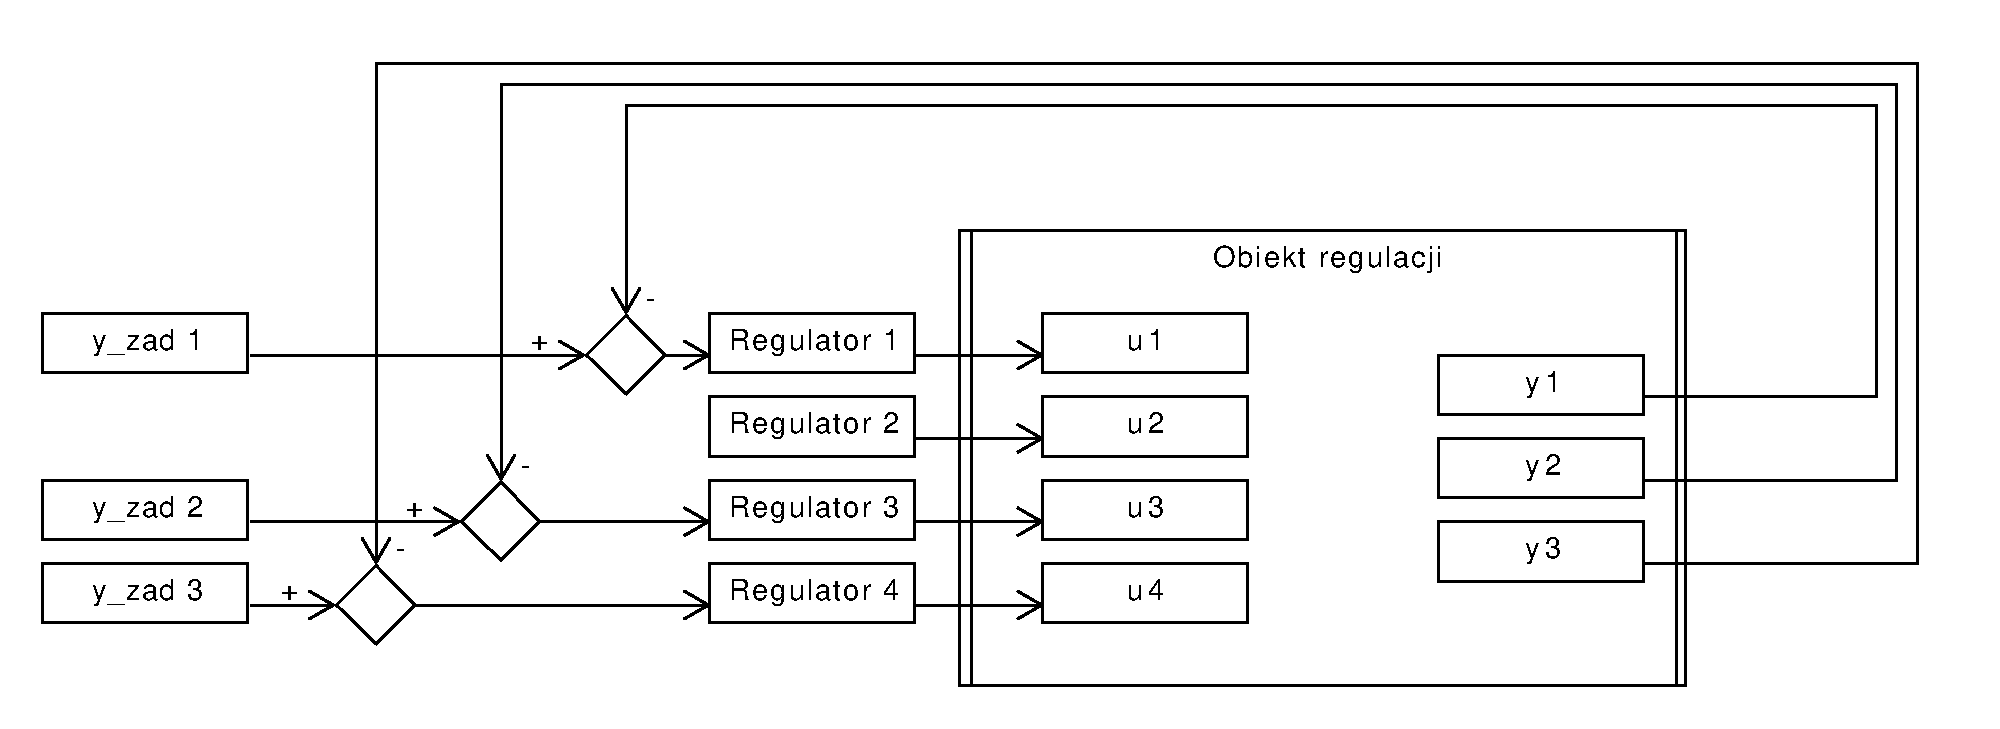
\includegraphics[scale=0.7, angle=90]{uklad_regulacji_pid.pdf}
\caption{Struktura regulacji opisywana przez macierz z listingu \ref{pro_pid_conn_matrix}}
\end{figure}

\FloatBarrier

Mając gotową opisaną strukturę regulatora wielowymiarowego oraz dobrane parametry,
możliwa jest implementacja pętli obliczającej nowe sterowania. \\

\begin{lstlisting}[style=custommatlab,frame=single,label={pro_pid_petla},caption={Pętla obliczająca sterowania wielowymiarowego regulatora PID},captionpos=b]
%% Petla symulujaca dzialanie cyfrowego algorytmu PID w wersji MIMO
for k = 5:SIM_LEN  
  [y1, y2, y3] = symulacja_obiektu1(inputs(k-1, 1), inputs(k-2, 1), ...
                                    inputs(k-3, 1), inputs(k-4, 1), ...
                                    inputs(k-1, 2), inputs(k-2, 2), ...
                                    inputs(k-3, 2), inputs(k-4, 2), ...
                                    inputs(k-1, 3), inputs(k-2, 3), ...
                                    inputs(k-3, 3), inputs(k-4, 3), ...
                                    inputs(k-1, 4), inputs(k-2, 4), ...
                                    inputs(k-3, 4), inputs(k-4, 4), ...
                                    outputs(k-1, 1), outputs(k-2, 1), ...
                                    outputs(k-3, 1), outputs(k-4, 1), ...
                                    outputs(k-1, 2), outputs(k-2, 2), ...
                                    outputs(k-3, 2), outputs(k-4, 2), ...
                                    outputs(k-1, 3), outputs(k-2, 3), ...
                                    outputs(k-3, 3), outputs(k-4, 3));
  outputs(k, :) = [y1 y2 y3];                        
  errors(k, :) = setpoints(k, :) - outputs(k, :); % obliczenie uchybow    

  % obliczenie nowych sterowan
  for i=1:N
    error = CONNECTION_MATRIX(i,:)*(errors(k-2:k, :)');
    inputs(k,i) = r2(i)*error(1) + r1(i)*error(2) + ...
                  r0(i)*error(3) + inputs(k-1, i); 
  end
end
\end{lstlisting}

\section{Strojenie wielowymiarowego regulatora PID z binarną macierzą połączeń}
\label{pro_pid_bin_conn}

Strojenie wielowymiarowego regulatora PID nie należy do spraw prostych.
W dalszej części tej sekcji opisaliśmy proces eksperymentalnego 
doboru parametrów regulatora.

\subsection{Konfiguracja z najmocniejszymi wzmocnieniami}
\label{pro_pid_konf1}

Analizując odpowiedzi na poszczególne skoki sygnałów wejściowych, zdecydowaliśmy się
sprawdzić konfigurację wejść i wyjść w której:\\

\begin{itemize}
    \item uchyb wyjścia pierwszego wchodzi na wejście drugie
    \item uchyb wyjścia drugiego wchodzi na wejście pierwszego
    \item uchyb wyjścia trzeciego wchodzi na wejście trzeciego
    \item wejście czwarte pozostaje niesterowane
\end{itemize}

\noindent Macierz połączeń w tym przypadku miała postać: \\
\[
C =
\begin{bmatrix}
    0 & 1 & 0 \\
    1 & 0 & 0 \\
    0 & 0 & 1 \\
    0 & 0 & 0 
\end{bmatrix}
\]


